\documentclass[11pt]{amsart}
\usepackage[margin=1.15in]{geometry}
\usepackage{amsmath,amssymb,amsthm,graphicx,booktabs}
\usepackage[colorlinks=true,allcolors=blue]{hyperref}
\newtheorem{theorem}{Theorem}
\newtheorem{corollary}[theorem]{Corollary}
\newtheorem{lemma}[theorem]{Lemma}
\newtheorem{proposition}[theorem]{Proposition}
\newtheorem{question}[theorem]{Question}
\theoremstyle{remark}
\newtheorem{remark}[theorem]{Remark}
\newcommand{\Dout}{D_{\mathrm{out}}}
\newcommand{\Din}{D_{\mathrm{in}}}
\newcommand{\yout}{y_{\mathrm{out}}}
\newcommand{\yin}{y_{\mathrm{in}}}

\begin{document}
\title[Whirling knight's tours with $n$ and with $n/2$ coils]{Whirling knight's tours\\ with $n$ coils and with $n/2$ coils}
\author{Zijian Zeng}
\address{UCSI University, Kuala Lumpur, Malaysia}
\date{16 November 2026. The results on $n$ coils were first obtained on 14 November 2026 and made public on
16 November; the construction for $n/2$ coils was obtained on 16 November 2026.}

\begin{abstract}
A whirling knight's tour of the $n\times n$ board, introduced by Knuth in a draft of \emph{The Art of Computer
Programming}, is a closed knight's tour in which every move turns counterclockwise about the centre of the board. Its
number of coils is its winding number about the centre, which lies between $n/2$ and $n$. Knuth's exercise
7.2.2.4--231 asks for tours with exactly $n/2$ coils and with exactly $n$ coils. Together with results of S.~Li and of N.~Beluhov and
F.~Stappers, the present note settles both questions.
\begin{itemize}
\item \emph{$n$ coils.} Such a tour exists if and only if $n=3$, or $n\ge12$ and $4\mid n$. We prove that none
exists for $n\ge5$ unless $4$ divides $n$, by a short weighted counting argument, and we give tours for $n=16$, $20$
and $24$. For $n\ge52$ the existence part rests on the construction reported in Knuth's draft.
\item \emph{$n/2$ coils.} Such a tour exists if and only if $n\ge16$ and $n\equiv0$ or $2\pmod 8$. Nonexistence
is due to S.~Li and to exhaustive counts. We prove existence: there are explicit tours for $n\le90$, and for
$n\ge96$ the tour is built from one of six seed tours, whose outer ring of width $12$ can be stretched and nested.
\end{itemize}
All tours are verified in exact arithmetic by an independent program, and the general construction rests on a finite
list of conditions on the six seeds that a program checks.
\end{abstract}
\maketitle

\section{Introduction}

In the draft of Section 7.2.2.4 of \emph{The Art of Computer Programming}~\cite{knuth}, Knuth introduces the
following variant of the knight's tour (exercises 227--232).

\subsection*{Definitions}
Take the cells $(i,j)$ with $0\le i,j<n$, where $i$ is the row and $j$ the column, and let the \emph{pivot} be the centre $\bigl(\tfrac{n-1}2,\tfrac{n-1}2\bigr)$
of the board. When $n$ is odd the central cell is removed. We use centred coordinates
$x=i-\tfrac{n-1}2$ and $y=j-\tfrac{n-1}2$, so the pivot is the origin. For cells $u=(x_u,y_u)$ and $w=(x_w,y_w)$
write $u\times w=x_uy_w-x_wy_u$.
\begin{itemize}
\item There is an \emph{arc} $u\to w$ when $w-u$ is a knight move and $u\times w>0$. This is the condition of
\cite[answer 227]{knuth}: the move turns counterclockwise about the pivot.
\item A \emph{whirling knight's tour} is a Hamiltonian cycle of this digraph.
\item Its number of \emph{coils} is its winding number about the pivot. Since every arc turns the same way, this is
the number of times the tour passes the direction of a plumb-line above the pivot, inside a move or at a cell; that
is the definition in \cite[exercise 229]{knuth}.
\end{itemize}

\subsection*{What was known}
All of the following is reported in \cite{knuth}.
\begin{itemize}
\item A tour of the $n\times n$ board has at least $n/2$ and at most $n$ coils (exercise 229(c)). Exercise 231
asks for tours that attain these bounds: (a) $n/2$ coils, (b) $n$ coils. For even $n$ the lower bound is easy to
see: a diagonal half-line from the pivot contains $n/2$ cells, and the tour passes its direction once at each of
them.
\item Exhaustive counts for $n\le 11$ (answer 229). In particular no $n\times n$ tour has $n$ coils for
$4\le n\le 11$, and the unique $3\times3$ tour has $3$ coils.
\item A $12\times12$ tour with $12$ coils, found by N.~Beluhov with integer programming (answer 231).
\item Tours with $n$ coils for every multiple of $4$ with $n\ge28$, by a construction of N.~Beluhov and F.~Stappers
(answer 232).
\item Tours with $n/2$ coils for $n=16$ and $n=18$ (answer 231).
\end{itemize}
In addition, S.~Li~\cite{li} proved that no tour has $n/2$ coils when $n\equiv4$ or $6\pmod 8$, by exhibiting
closed-form Farkas certificates for a linear relaxation. This settled a conjecture of Beluhov; Li remarks that the
other two classes admit such tours, with the examples $n=16$ and $n=18$. To our knowledge the following were open:
the cases $13\le n\le27$ of exercise 231(b); all $n\ge29$ that are not multiples of $4$; and, for $n/2$ coils, every
$n\ge24$ with $n\equiv0$ or $2\pmod 8$. We could not rule out that a construction for $n/2$ coils is known to others
but unpublished; the draft \cite{knuth} of 8 May 2026 contains none.

\subsection*{Results}
\begin{theorem}\label{thm:main}
Let $n\ge5$ with $n\not\equiv0\pmod4$. Then no $n\times n$ whirling knight's tour has exactly $n$ coils.
\end{theorem}

\begin{corollary}\label{cor:iff}
An $n\times n$ whirling knight's tour with exactly $n$ coils exists if and only if $n=3$, or $n\ge12$ and $4\mid n$.
\end{corollary}
\begin{proof}
\emph{Nonexistence.} For $n=1$ and $n=2$ the digraph has no arcs. Theorem~\ref{thm:main} covers every $n\ge5$ that
is not a multiple of $4$. The cases $n=4$ and
$n=8$ are excluded by the exhaustive counts in \cite[answer 229]{knuth}, which we reproduced (Section~\ref{sec:comp}).

\emph{Existence.} The $3\times3$ knight cycle around the removed centre has $3$ coils. For $n=12$ there is Beluhov's
tour. For $n=16,20,24$ we give tours in Section~\ref{sec:comp}. For $n\ge28$ there is the construction of
\cite[answer 232]{knuth}. Independently of that construction, Section~\ref{sec:comp} also gives a tour for every
multiple of $4$ with $12\le n\le48$.
\end{proof}

\begin{remark}
Exercise 231 of \cite{knuth} remarks that no tour with $n$ coils exists when $n<12$. Read literally, this overlooks
$n=3$: answer
229(d) of the same draft records the single $3\times3$ tour, which has $3$ coils.
\end{remark}

For the least possible number of coils we prove the following.
\begin{theorem}\label{thm:half}
For every $n\ge16$ with $n\equiv0$ or $2\pmod 8$ there is an $n\times n$ whirling knight's tour with exactly $n/2$
coils.
\end{theorem}

\begin{corollary}\label{cor:half}
Let $n$ be even. An $n\times n$ whirling knight's tour with exactly $n/2$ coils exists if and only if $n\ge16$ and
$n\equiv0$ or $2\pmod 8$.
\end{corollary}
\begin{proof}
Existence is Theorem~\ref{thm:half}. For $n\equiv4$ or $6\pmod 8$ nonexistence is Li's theorem~\cite{li}. For $n=2$
the digraph has no arcs. For $n=8$ and $n=10$ it follows from the exhaustive counts in \cite[answer 229]{knuth}; our
own search also finds no such tour (Section~\ref{sec:comp}).
\end{proof}
The cases $n=16$ and $n=18$ of Theorem~\ref{thm:half} were known \cite[answer 231]{knuth}; the theorem is new for
$n\ge24$. Its proof is computer-assisted: it rests on $26$ tours, given in the accompanying files, and on a finite
check carried out by a program.

The proof of Theorem~\ref{thm:half} is in Section~\ref{sec:half}. For $n\le90$ we list tours. For larger $n$ the
tour consists of nested rings of width $12$ around a tour of side between $72$ and $90$. Each ring is a path that
is periodic along parts of each side, so that it can be lengthened to fit any larger board in the same class
modulo $24$.

\section{The counting identity}

\begin{lemma}\label{lem:rays}
Let $R$ be an open ray from the pivot that contains no cell. A whirling knight's tour with $c$ coils contains exactly
$c$ arcs that cross $R$, and no arc crosses $R$ twice.
\end{lemma}
\begin{proof}
For an arc $u\to w$ we have $u\times w\ne0$, so the segment from $u$ to $w$ misses the pivot, and $u\times w>0$ means
that the polar angle increases along the segment, by a total amount in $(0,\pi)$. So the angle increases monotonically
along the whole tour, by $2\pi c$ in all, and it passes the direction of $R$ exactly $c$ times. Each passage happens
inside an arc, because $R$ contains no cell.
\end{proof}

\begin{lemma}\label{lem:count}
Let $R_1,\dots,R_4$ be rays as in Lemma~\ref{lem:rays}, and let $\yout$ and $\yin$ be real functions on the cells. For
an arc $a=u\to w$ let $k(a)$ be the number of rays among $R_1,\dots,R_4$ that $a$ crosses, and put
\[ g(a)=\yout(u)+\yin(w)+k(a). \]
Then every whirling knight's tour $T$ with $c$ coils satisfies
\[ \sum_{a\in T}g(a)=\sum_{v}\bigl(\yout(v)+\yin(v)\bigr)+4c. \]
\end{lemma}
\begin{proof}
Every cell is the tail of exactly one arc of $T$ and the head of exactly one. By Lemma~\ref{lem:rays}, each ray is
crossed by exactly $c$ arcs of $T$.
\end{proof}

To prove Theorem~\ref{thm:main} we take $c=n$ and choose rays and weights with $g(a)\le0$ for every arc, while the
right-hand side is positive. All sets below are invariant under the quarter turn $\rho\colon(i,j)\mapsto(j,n-1-i)$,
which is $(x,y)\mapsto(y,-x)$ in centred coordinates. The digraph is invariant under $\rho$. For a set $A$ of cells,
its \emph{orbit} is $A\cup\rho A\cup\rho^2A\cup\rho^3A$.

\section{Proof for \texorpdfstring{$n\equiv2\pmod4$}{n = 2 (mod 4)}}

Let $n=2h$ with $h\ge3$ odd. We use the original coordinates $(i,j)$.
\begin{itemize}
\item \emph{Rays.} The four half-lines from the pivot along the two central grid lines, that is, between rows $h-1$
and $h$ and between columns $h-1$ and $h$. They contain no cell.
\item \emph{Colouring.} $\kappa(i,j)=\bigl(i+j+[i<h]+[j<h]\bigr)\bmod 2$. This is a checkerboard colouring in each
quadrant, mirrored across the central lines. It is $\rho$-invariant because $n$ is even.
\item \emph{Corrections.} $X$ is the orbit of $\{(i,h): i\text{ odd},\ 1\le i\le h-2\}$ and $Y$ is the orbit of
$\{(i,h-1): i\text{ odd},\ 1\le i\le h-2\}$.
\item \emph{Weights.} $\yout(v)=[\kappa(v)=1]-2[v\in X]$ and $\yin(v)=-[\kappa(v)=0]-2[v\in Y]$.
\end{itemize}

\begin{lemma}\label{lem:even}
With these choices, $g(a)\le0$ for every arc $a=u\to w$.
\end{lemma}
\begin{proof}
A knight move changes the parity of $i+j$. It crosses each central line at most once, and it never passes through the
pivot. So $k(a)$ is the number of central lines that $a$ crosses, and $\kappa(u)\ne\kappa(w)$ exactly when $k(a)$ is
even. Write $g(a)=b(a)-2[u\in X]-2[w\in Y]$ with $b(a)=[\kappa(u)=1]-[\kappa(w)=0]+k(a)$.

\emph{Case $k(a)=0$.} Then $\kappa(w)\ne\kappa(u)$, so $b(a)=0$ and $g(a)\le0$.

\emph{Case $k(a)=1$.} Then $\kappa(w)=\kappa(u)$. If $\kappa(u)=0$, then $b(a)=0-1+1=0$. If $\kappa(u)=1$, then
$b(a)=2$, and we must show that $u\in X$ or $w\in Y$. By symmetry we may assume that $a$ crosses the ray pointing to
row $0$. Then both endpoints lie in rows less than $h$. The condition $u\times w>0$ forces $a$ to go from a column
$\ge h$ to a column $\le h-1$, so there are two possibilities.
\begin{itemize}
\item $u=(i,h)$. Here $\kappa(u)=(i+h+1)\bmod2=i\bmod2$, since $h$ is odd. So $i$ is odd, and $i<h$ gives
$1\le i\le h-2$. Hence $u\in X$.
\item $u=(i,h+1)$ and $w=(i\pm1,h-1)$. Here $\kappa(u)=(i+h+2)\bmod 2=(i+1)\bmod 2$, so $i$ is even. The row of $w$ is
odd and less than $h$, so it lies in $[1,h-2]$. Hence $w\in Y$.
\end{itemize}

\emph{Case $k(a)=2$.} Then $b(a)=2$ and $a$ joins opposite quadrants. One coordinate changes by $1$ and the other by
$2$, so in centred coordinates one endpoint is $(\frac\sigma2,\frac\tau2)$ with $\sigma,\tau\in\{1,-1\}$, and the
other is $(-\frac\sigma2,-\frac{3\tau}2)$ or $(-\frac{3\sigma}2,-\frac\tau2)$. Exactly eight such arcs satisfy $u\times w>0$. They are listed in Table~\ref{tab:central},
and each has $u\in X$ or $w\in Y$.
\end{proof}

\begin{table}[h]
\caption{The eight arcs that cross both central lines when $n\equiv2\pmod 4$, in centred coordinates $(x,y)$.
The cell $(-\frac32,\frac12)$ is $(h-2,h)\in X$, and $(-\frac32,-\frac12)$ is $(h-2,h-1)\in Y$.}
\label{tab:central}
\begin{tabular}{lcl@{\qquad}lcl}
\toprule
\multicolumn{3}{c}{$u\in X$} & \multicolumn{3}{c}{$w\in Y$}\\
\midrule
$(-\frac32,\frac12)$&$\to$&$(\frac12,-\frac12)$ & $(\frac12,\frac12)$&$\to$&$(-\frac32,-\frac12)$\\
$(\frac12,\frac32)$&$\to$&$(-\frac12,-\frac12)$ & $(\frac12,-\frac12)$&$\to$&$(-\frac12,\frac32)$\\
$(\frac32,-\frac12)$&$\to$&$(-\frac12,\frac12)$ & $(-\frac12,-\frac12)$&$\to$&$(\frac32,\frac12)$\\
$(-\frac12,-\frac32)$&$\to$&$(\frac12,\frac12)$ & $(-\frac12,\frac12)$&$\to$&$(\frac12,-\frac32)$\\
\bottomrule
\end{tabular}
\end{table}

\begin{proof}[Proof of Theorem~\ref{thm:main} for $n\equiv 2\pmod 4$]
Each quadrant is an $h\times h$ square with $h$ odd, and $\kappa$ is a checkerboard colouring of it whose corner
cells at the outer corner of the board have $\kappa=0$. So each quadrant has one more cell with $\kappa=0$ than with
$\kappa=1$, and $\sum_v\bigl([\kappa(v)=1]-[\kappa(v)=0]\bigr)=-4$. The four rotated copies in the definitions of
$X$ and $Y$ lie in different arms, so they are disjoint and $|X|=|Y|=4\cdot\frac{h-1}2$. With $c=n$,
the right-hand side of Lemma~\ref{lem:count} is
\[ -4-2|X|-2|Y|+4n=-4-8(h-1)+8h=4>0, \]
while the left-hand side is at most $0$ by Lemma~\ref{lem:even}. So no tour with $n$ coils exists.
\end{proof}

\section{Proof for odd \texorpdfstring{$n$}{n}}

Let $n=2m+1$ with $m\ge2$. In centred coordinates the cells are the integer points of $[-m,m]^2$ other than the
origin. Fix $0<\varepsilon<1/m$.
\begin{itemize}
\item \emph{Rays.} $R_N=\{t(-1,\varepsilon):t>0\}$ and its images under $\rho$. They contain no cell.
\item \emph{The cross.} $C$ is the set of cells with $x=0$ or $y=0$, so $|C|=4m$.
\item \emph{Corrections.} $P$ is the orbit of $\{(x,1): x<0,\ x\equiv m+1 \pmod 2\}$ and $Q$ is the orbit of
$\{(x,-1): x<0,\ x\equiv m+1\pmod 2\}$. Let $S$ be the set of the $8$ cells adjacent to the origin.
\item \emph{Sets.} $\Din=C\cup Q$. If $m$ is even, $\Dout=P$. If $m$ is odd, $\Dout=P\cup S$.
\item \emph{Weights.} $\yout(v)=[x+y\text{ odd}]-[v\in\Dout]$ and $\yin(v)=-[x+y\text{ even}]-[v\in\Din]$.
\end{itemize}
A knight move changes the parity of $x+y$, so the checkerboard terms cancel on every arc, and
\[ g(a)=k(a)-[u\in\Dout]-[w\in\Din]\qquad\text{for every arc }a=u\to w. \]
When $m$ is odd we use $g'(a)=g(a)+[u\in S,\ w\notin S]$ instead.

\begin{lemma}\label{lem:north}
Let $a=u\to w$ be an arc that crosses $R_N$. Then $u\in\Dout$ or $w\in\Din$. If $m$ is odd and $a$ leaves $S$
(that is, $u\in S$ and $w\notin S$), then $w\in\Din$.
\end{lemma}
\begin{proof}
Let $s(x,y)=y+\varepsilon x$. Since $|\varepsilon x|<1$ on cells, a cell has $s>0$ exactly when $y\ge1$, or $y=0$ and
$x>0$. The arc crosses the line $s=0$ from $s>0$ to $s<0$, at a point with $x<0$. If $y_u=0$, then $x_u>0$, and
$u\times w=x_uy_w>0$ forces $y_w\ge1$, so $s(w)>0$, which is impossible. Hence $y_u\ge1$, and then $y_w\ge -1$.
\begin{itemize}
\item If $y_w=0$, then $x_w<0$ and $w\in C\subseteq\Din$.
\item Otherwise $y_u=1$, $y_w=-1$ and $x_w=x_u\pm1$. The segment meets the line $s=0$ at the point with
$x=(x_u+x_w)/\bigl(2-\varepsilon(x_w-x_u)\bigr)$, which is negative exactly when $x_u+x_w\le-1$. So both
$x_u,x_w\le0$. Exactly one of $x_u,x_w$ is congruent to $m+1$ modulo $2$; call it $x^*$.
If $x^*<0$, then $u\in P$ or $w\in Q$. If $x^*=0$, then $m$ is odd, and either $u=(0,1)\in S\subseteq\Dout$ or
$w=(0,-1)\in C$.
\end{itemize}
For the last claim, let $m$ be odd and let $a$ leave $S$. Then $u\in\{(-1,1),(0,1),(1,1)\}$, and going through the
knight moves from these cells shows that $a$ is one of
\[ (-1,1)\to(-3,0),\qquad (-1,1)\to(-2,-1),\qquad (0,1)\to(-2,0). \]
The heads $(-3,0)$ and $(-2,0)$ are in $C$, and $(-2,-1)\in Q$ because $-2\equiv m+1\pmod 2$.
\end{proof}

\begin{lemma}\label{lem:odd}
If $m$ is even, $g(a)\le0$ for every arc. If $m$ is odd, $g'(a)\le0$ for every arc.
\end{lemma}
\begin{proof}
\emph{Case $k(a)=0$.} Then $g(a)\le0$. If $m$ is odd and $a$ leaves $S$, then $u\in S\subseteq\Dout$, so $g'(a)\le0$.

\emph{Case $k(a)=1$.} By symmetry $a$ crosses $R_N$, and Lemma~\ref{lem:north} gives $g(a)\le0$. If $m$ is odd and $a$
leaves $S$, then $u\in\Dout$ and $w\in\Din$ by Lemma~\ref{lem:north}, so $g'(a)=1-1-1+1=0$.

\emph{Case $k(a)\ge2$.} Two of the rays are at least a quarter turn apart, so the angle from $u$ to $w$ exceeds
$\pi/2$. Then $u\cdot w<0$, so $|u|^2+|w|^2<|u-w|^2=5$, and $u\cdot w=\frac12(|u|^2+|w|^2-5)$ is an integer. The only
possibility is $\{|u|^2,|w|^2\}=\{1,2\}$: one endpoint is an axis neighbour of the origin and the other a diagonal
neighbour. Checking these arcs, the ones that cross two rays are
\[ (1,1)\to(-1,0)\quad\text{and its three images under }\rho, \]
and none crosses three. Here $w\in C$. The tail is a diagonal neighbour: it lies in $P$ when $m$ is even (take
$x=-1$), and in $S$ when $m$ is odd. So $g(a)=2-1-1=0$, and these arcs do not leave $S$.
\end{proof}

\begin{proof}[Proof of Theorem~\ref{thm:main} for odd $n$]
The removed centre has $x+y$ even, so the remaining cells have equally many odd and even values of $x+y$, and the
checkerboard terms sum to $0$. The sets in the definitions of $P$ and $Q$ have $m/2$ elements when $m$ is even and
$(m-1)/2$ when $m$ is odd, and their four rotated copies are pairwise disjoint. Also $Q\cap C=\emptyset$, and
$P\cap S=\emptyset$ when $m$ is odd.

\emph{$m$ even.} $|\Dout|=2m$ and $|\Din|=4m+2m$. By Lemma~\ref{lem:count} with $c=n$, a tour with $n$ coils would have
$\sum_{a\in T}g(a)=4n-8m=4>0$, contradicting Lemma~\ref{lem:odd}.

\emph{$m$ odd.} $|\Dout|=2(m-1)+8$ and $|\Din|=4m+2(m-1)$, so $\sum_{a\in T}g(a)=4n-8m-4=0$. A tour visits cells
outside $S$, so at least one of its arcs leaves $S$. Hence $\sum_{a\in T}g'(a)\ge1$, contradicting
Lemma~\ref{lem:odd}.
\end{proof}

\begin{remark}
When $4\mid n$ the same construction gives no contradiction, as it must. With $h=n/2$ even, each quadrant has
equally many cells of each colour, and each arm needs $h/2$ corrected cells per column instead of $(h-1)/2$. The
value $4$ becomes $0$.
\end{remark}

\begin{remark}
The weights were found by computer, following the method of Li~\cite{li}. For $13\le n\le27$ we solved the linear
relaxation ``a fractional cycle cover in which every ray is crossed $n$ times'' and extracted rational Farkas
certificates. Restricting the certificates to be
rotation-invariant, to use only four rays, and to differ from a checkerboard only near the central cross produced the
patterns above, which we then proved for all $n$.
\end{remark}

\section{Tours with \texorpdfstring{$n/2$}{n/2} coils}\label{sec:half}

In this section every board has even side. A set of arcs in which each cell has at most one successor is described by
its \emph{moves} $m(z)=\operatorname{succ}(z)-z$. We write $c(z)$ for the column of a cell $z$.

\subsection*{Rings and seeds}
The \emph{depth} of a cell $(i,j)$ of the $N\times N$ board is $\min(i,j,N-1-i,N-1-j)$. The \emph{ring} is the set
of cells of depth less than $12$, and the other cells form the \emph{inner board}. The translation by $(12,12)$ maps
the $(N-24)\times(N-24)$ board onto the inner board and the pivot to the pivot, so it preserves arcs and coils.

A \emph{seed} is a pair $(T_0,T_1)$ with the following properties.
\begin{itemize}
\item $T_0$ is a whirling tour of the $N_0\times N_0$ board with $N_0/2$ coils.
\item $T_1$ is a whirling tour of the $N_1\times N_1$ board with $N_1/2$ coils, where $N_1=N_0+24$.
\item $T_1$ contains every arc of $T_0+(12,12)$ except one arc $u\to v$.
\end{itemize}
The remaining arcs of $T_1$ then form a path $P$ from $u$ to $v$ that visits every cell of the ring. We call $P$ the
\emph{ring path}. It is a Hamiltonian path of the set $G$ that consists of the ring and the two cells $u$ and $v$.
Figure~\ref{fig:ring} shows a seed with $N_1=96$.

\subsection*{Inserting a period}
The next lemma lets us lengthen a path where it is periodic. For a cell $z$ and a fixed integer $\tau\ge1$ write
$z^+=z+(0,\tau)$ and $z^-=z-(0,\tau)$.

\begin{lemma}\label{lem:insert}
Let $G$ be a finite set of cells, that is, of points of $\mathbb Z^2$, and $P$ a Hamiltonian path of $G$ from $s$
to $t$ whose arcs are knight moves, with moves $m$. Let $A<B$ and $\tau\ge1$ be integers with $B-A\ge\tau+4$. Assume:
\begin{itemize}
\item[(a)] $c(s)$ and $c(t)$ are not in $[A,B)$. For every cell $z$ with $A\le c(z)<B-\tau$ we have
$z\in G\iff z^+\in G$, and $m(z)=m(z^+)$ when both are in $G$.
\item[(b)] If $z\in G$ and $A\le c(z)<A+2$, the part of $P$ between $z$ and $z^+$ lies in columns less than $B$.
\item[(c)] If $z\in G$ and $B-2\le c(z)<B$, the part of $P$ between $z^-$ and $z$ lies in columns at least $A$.
\end{itemize}
Let $G'=\{z\in G:c(z)<B\}\cup\{z^+:z\in G,\ c(z)\ge A\}$. For $z\in G'$ put $m'(z)=m(z)$ if $c(z)<B$, and
$m'(z)=m(z^-)$ if $c(z)\ge A+\tau$. Then $m'$ is well defined at every cell of $G'$ other than $t'$, and the arcs $z\to z+m'(z)$ form a Hamiltonian
path
$P'$ of $G'$ from $s'$ to $t'$, where $x'=x$ if $c(x)<A$ and $x'=x^+$ if $c(x)\ge B$. Moreover \textup{(a)--(c)} hold
for $G'$ and $P'$ with $B+\tau$ in place of $B$.
\end{lemma}
\begin{proof}
Let $W=\{z\in G':c(z)<B\}$ and $E=\{z\in G':c(z)\ge A+\tau\}$. By (a), $W=\{z\in G:c(z)<B\}$ and
$E=\{z^+:z\in G,\ c(z)\ge A\}$. On $W\cap E$ the two definitions of $m'$ agree, again by (a). So $m'=m$ on $W$, and
$m'(z^+)=m(z)$ for $z^+\in E$. In words: on $W$ the new arcs are the old ones, and on $E$ they are the old arcs
between cells of column at least $A$, translated by $(0,\tau)$.

A knight move changes the column by at most $2$, and $B-(A+\tau)\ge4$. Hence for every cell $z$ the five columns
$c(z)-2,\dots,c(z)+2$ are all less than $B$, or all at least $A+\tau$. In the first case call $z$ itself the
\emph{counterpart} of $z$; otherwise call $z^-$ its counterpart. All arcs of $P$ at the counterpart, and all arcs of
$P'$ at $z$, then lie in $W$, respectively in $E$ after translation. So $z+m'(z)\in G'$, and $z$ has as many
incoming and outgoing arcs in $P'$ as its counterpart has in $P$. Exactly one cell of $G'$ has counterpart $s$, namely
$s'$, and exactly one has counterpart $t$, namely $t'$; this is because $c(s)$ and $c(t)$ are not in $[A,B)$. Therefore $P'$ consists of a path from $s'$ to $t'$ and
possibly some cycles.

To exclude cycles, call a cell of $G'$ \emph{good} if $P'$ joins it to $s'$, directions ignored. Let
$P=(x_0,x_1,\dots,x_M)$ with $x_0=s$. We show by induction on $i$:
\begin{itemize}
\item[(1)] if $c(x_i)<B$, then $x_i$ is good;
\item[(2)] if $c(x_i)\ge A$, then $x_i^+$ is good.
\end{itemize}
For $i=0$ one statement is void and the other says that $s'$ is good. Let $y=x_{i+1}$ and assume (1) and (2) for
$x_i$.
\begin{itemize}
\item \emph{$c(y)<B$ and $c(x_i)<B$.} The arc $x_i\to y$ lies in $W$, so $y$ is good.
\item \emph{$c(y)<B\le c(x_i)$.} Then $c(y)\ge B-2\ge A$. The arc $x_i^+\to y^+$ lies in $E$, so $y^+$ is good. By
(c), $y^-$ and $y$ are joined in $P$ through cells of column at least $A$. Translating, $y$ and $y^+$ are joined in
$P'$. So $y$ is good.
\item \emph{$c(y)\ge A$ and $c(x_i)\ge A$.} The arc $x_i^+\to y^+$ lies in $E$, so $y^+$ is good.
\item \emph{$c(y)\ge A>c(x_i)$.} Then $c(y)<A+2<B$, and $y$ is good by the first case. By (b), $y$ and $y^+$ are
joined in $P$ through cells of column less than $B$, hence also in $P'$. So $y^+$ is good.
\end{itemize}
Every cell of $G'$ is some $x_i$ with $c(x_i)<B$ or some $x_i^+$ with $c(x_i)\ge A$. So all cells are good and $P'$
is a single path.

Finally we check (a)--(c) for $G'$, $P'$ and the interval $[A,B+\tau)$. The columns of $s'$ and $t'$ are less
than $A$ or at least $B+\tau$. If $A\le c(z)<B$ then
$z\in G'\iff z\in G\iff z^+\in G'$, and $m'(z^+)=m(z)=m'(z)$; this is (a). In (b) the part of $P$ between $z$ and
$z^+$ lies in $W$, so it is also a part of $P'$. In (c) we have $z=y^+$ with $B-2\le c(y)<B$, and the part of $P$
between $y^-$ and $y$, translated, is the part of $P'$ between $z^-$ and $z$.
\end{proof}

The lemma also holds with rows in place of columns. We call the interval $[A,B)$ together with $\tau$ a
\emph{zone}, and the passage from $(G,P)$ to $(G',P')$ an \emph{insertion}. After $q$ insertions in the same zone,
the moves in columns less than $B$ are unchanged, the moves in columns at least $A+q\tau$ are the old ones
translated by $(0,q\tau)$, and in the columns from $A$ to $B+q\tau-1$ the moves are periodic with period $\tau$.

\subsection*{Stretching a seed}
Fix a seed and put $a=19$, $h=N_1/2$ and $b=N_1-19$. For $e\ge0$ let $N_{e+1}=N_1+24e$. Define
$\varphi_e\colon\{0,\dots,N_1-1\}\to\{0,\dots,N_{e+1}-1\}$ by
\[ \varphi_e(t)=\begin{cases} t & t<a,\\ t+6e & a\le t<h,\\ t+18e & h\le t<b,\\ t+24e & t\ge b.\end{cases} \]
Its image omits three blocks of $6e$, $12e$ and $6e$ consecutive integers, which begin at $a$, at $h+6e$ and at
$b+18e$. Define $\pi_e\colon\{0,\dots,N_{e+1}-1\}\to\{0,\dots,N_1-1\}$ by $\pi_e(\varphi_e(t))=t$ and, for $s$ in a
block,
\[ \pi_e(s)\in\{a-3,a-2,a-1\},\quad \pi_e(s)\in\{h-2,h-1\},\quad \pi_e(s)\in\{b,b+1,b+2\} \]
for the first, second and third block, with $\pi_e(s)\equiv s$ modulo $3$, $2$ and $3$ respectively. Both maps act
on cells coordinatewise. Then $\pi_e$ maps the ring of the $N_{e+1}\times N_{e+1}$ board onto the ring of the
$N_1\times N_1$ board.

Now define $T_{e+1}$ on the $N_{e+1}\times N_{e+1}$ board for $e\ge1$, given $T_e$:
\begin{itemize}
\item it contains every arc of $T_e+(12,12)$ except $\varphi_e(u)\to\varphi_e(v)$;
\item it contains the arc $\varphi_e(u)\to\varphi_e(u)+m(u)$;
\item every ring cell $z$ has the move $m(\pi_e(z))$.
\end{itemize}
Here $m$ denotes the moves of the ring path $P$ of the seed. For $e=0$ the same rule returns $T_1$.

\subsection*{Four finite conditions}
Let $D(t)$, for $0\le t<N_1$, be the set
\[\begin{array}{lll}
\{-12\}\ \ (t<a-3), & \{-12,-6\}\ \ (a-3\le t<a), & \{-6\}\ \ (a\le t<h-2),\\
\{-6,6\}\ \ (h-2\le t<h), & \{6\}\ \ (h\le t<b), & \{6,12\}\ \ (b\le t<b+3),\\
\{12\}\ \ (t\ge b+3).
\end{array}\]
We say that the seed is \emph{stretchable} if the following hold.
\begin{itemize}
\item[(Z)] Conditions (a), (b), (c) of Lemma~\ref{lem:insert} hold for $(G,P)$ and each of the three zones
\[ [14,21),\ \tau=3;\qquad [h-3,h+3),\ \tau=2;\qquad [N_1-21,N_1-14),\ \tau=3, \]
and also with rows in place of columns. Moreover, the parts of $P$ in (b) lie in columns (rows) at least $A-2$,
and those in (c) lie in columns (rows) less than $B+2$.
\item[(S)] $u=(r,c)$ and $v=(r',c')$ with $c,c'\in\{12,13\}$ and $25\le r,r'<h$, and $P$ contains the arc
$(r-6,c-12)\to(r'-6,c'-12)$.
\item[(W)] For every cell $z=(i,j)$ of $G$ other than $v$, with move $m(z)=(m_1,m_2)$, and for all
$\delta_1\in D(i)$ and $\delta_2\in D(j)$, we have $\delta_1m_2-m_1\delta_2\ge0$.
\item[(C)] Every cell $(i,j)$ with $i<12$ and $h-3\le j<h+3$ has move $(2,-1)$ or $(-2,-1)$.
\end{itemize}

\begin{proposition}\label{prop:stretch}
If the seed $(T_0,T_1)$ is stretchable, then for every $k\ge0$ the set $T_k$ is a whirling knight's tour of the
board of side $N_0+24k$, with $(N_0+24k)/2$ coils.
\end{proposition}
\begin{proof}
The cases $k=0$ and $k=1$ are part of the definition of a seed. Let $e\ge1$ and assume the claim for $T_e$.

\emph{The ring path.} Apply Lemma~\ref{lem:insert} to $(G,P)$: $2e$ insertions in the first zone, $6e$ in the
second and $2e$ in the third, for columns and then for rows. This is allowed, because the hypotheses (a)--(c) for one zone survive an insertion in
another zone. To see this, consider a column zone $[A,B)$. The ring cells in the columns $A-2,\dots,B+1$ belong to
the top side or to the bottom side of the ring. So each pair $z,z^+$ in (a) lies on one of these two sides. By (Z),
each part of $P$ in (b) or (c) stays in these columns. It does not contain $u$ or $v$, which are the ends of $P$,
and a knight move cannot lead from the top side to the bottom side; so the part also lies on one of the two sides.
An insertion in another column zone fixes all cells in the columns $A-2,\dots,B+1$, or translates all of them by the
same vector. An insertion in a row zone fixes the top side and translates the bottom side. The cells $u$ and $v$
stay in the columns $12$ and $13$, to the left of every column zone; their rows lie between the first and the
second row zone, and they are translated together with the second and third row zones. In each case (a)--(c)
still hold, for $[A,B)$ or for its translate. The same argument applies to the row zones. The result is a Hamiltonian path $P_e$ from $\varphi_e(u)$ to $\varphi_e(v)$ of the
set formed by the ring of the $N_{e+1}\times N_{e+1}$ board and these two cells. After the insertions the three column zones are
\[ [14,\,21+6e),\qquad [h-3+6e,\,h+3+18e),\qquad [N_1-21+18e,\,N_1-14+24e). \]
They contain the three blocks omitted by $\varphi_e$, and the values
of $\pi_e$ on a block lie in the original zone and in the right residue class. So by the remark after the lemma, the
move of $P_e$ at a ring cell $z$ is $m(\pi_e(z))$, and its move at $\varphi_e(u)$ is $m(u)$. So $T_{e+1}$ consists of
$T_e+(12,12)$ without the arc $\varphi_e(u)\to\varphi_e(v)$, together with $P_e$.

\emph{Hamiltonian cycle.} We claim that $T_e+(12,12)$ contains the arc $\varphi_e(u)\to\varphi_e(v)$; then
$T_{e+1}$ is a Hamiltonian cycle. By (S), $\varphi_e(u)=(r+6e,c)$ and $\varphi_e(v)=(r'+6e,c')$. For $e=1$ the claim
is the last part of (S). For $e\ge2$, the ring of $T_e$ carries the path $P_{e-1}$. The cells
$(r-6,c-12)$ and $(r'-6,c'-12)$ have rows in $[a,h)$ and columns less than $a$, so $\varphi_{e-1}$ moves both by
$(6(e-1),0)$, and $P_{e-1}$ contains the arc $(r+6e-12,c-12)\to(r'+6e-12,c'-12)$. Adding $(12,12)$ gives the claim.

\emph{Every arc turns counterclockwise.} For the arcs of $T_e+(12,12)$ this holds by induction. Let $z$ be a cell
of $P_e$ other than its last cell, let $x=\pi_e(z)$, with $x=u$ if $z=\varphi_e(u)$, and let $m=m(x)$ be their
common move. Let $o_e$ be the pivot of the $N_{e+1}\times N_{e+1}$ board, so that $o_0$ is the pivot of the
$N_1\times N_1$ board; both coordinates of $o_e$ exceed those of $o_0$ by $12e$. We claim that
\[ z-o_e=(x-o_0)+e\,(\delta_1,\delta_2)\qquad\text{with }\delta_1\in\operatorname{conv}D(x_1),\
\delta_2\in\operatorname{conv}D(x_2), \]
where $x=(x_1,x_2)$. For a coordinate $s$ of $z$ of the form $\varphi_e(t)$ this is clear from the definition of
$\varphi_e$: $s-12e-t$ is $-12e$, $-6e$, $6e$ or $12e$. For $s$ in the first block, $t=\pi_e(s)\in\{a-3,a-2,a-1\}$
and $3\le s-t\le6e$, so $s-12e-t\in[-12e,-6e]$. For the second block, $6e+2\le s-t\le18e$, and for the third,
$18e\le s-t\le24e-3$. Since the cross product is bilinear,
\[ (z-o_e)\times m=(x-o_0)\times m+e\,(\delta_1m_2-m_1\delta_2). \]
The first term is positive because $T_1$ is whirling. The second is affine in $\delta_1$ and in $\delta_2$, and it is
nonnegative at the corners by (W), hence nonnegative.

\emph{Coils.} By Lemma~\ref{lem:rays} the number of coils of $T_{e+1}$ is the number of its arcs that cross the
half-line $R$ from the pivot along the central line towards row $0$, between the columns $h+12e-1$ and $h+12e$.
The arcs of $T_e+(12,12)$ cross it $N_e/2$ times, and the removed arc is not among them. An arc of $P_e$ that crosses
$R$ joins two cells in rows less than $12$ on different sides of the central line. These cells lie in the second
zone, where by (C) and periodicity every move is $(\pm2,-1)$. So exactly the $12$ cells of column $h+12e$ in rows
$0,\dots,11$ send an arc across $R$. Hence $T_{e+1}$ has $N_e/2+12=N_{e+1}/2$ coils.
\end{proof}

\begin{proof}[Proof of Theorem~\ref{thm:half}]
For $n\le90$ the tours are in an accompanying file (Section~\ref{sec:comp}). Every admissible $n\ge96$ is
$N_1+24(k-1)$ for a unique $N_1\in\{96,98,104,106,112,114\}$ and $k\ge1$. For each of these six values,
Section~\ref{sec:comp} gives a tour $T_1$ that forms a seed with the listed tour $T_0$ of side $N_1-24$. The
accompanying program checks, in exact integer arithmetic, that the six seeds are stretchable.
Proposition~\ref{prop:stretch} then gives $T_k$.
\end{proof}

\begin{figure}[t]
\centering
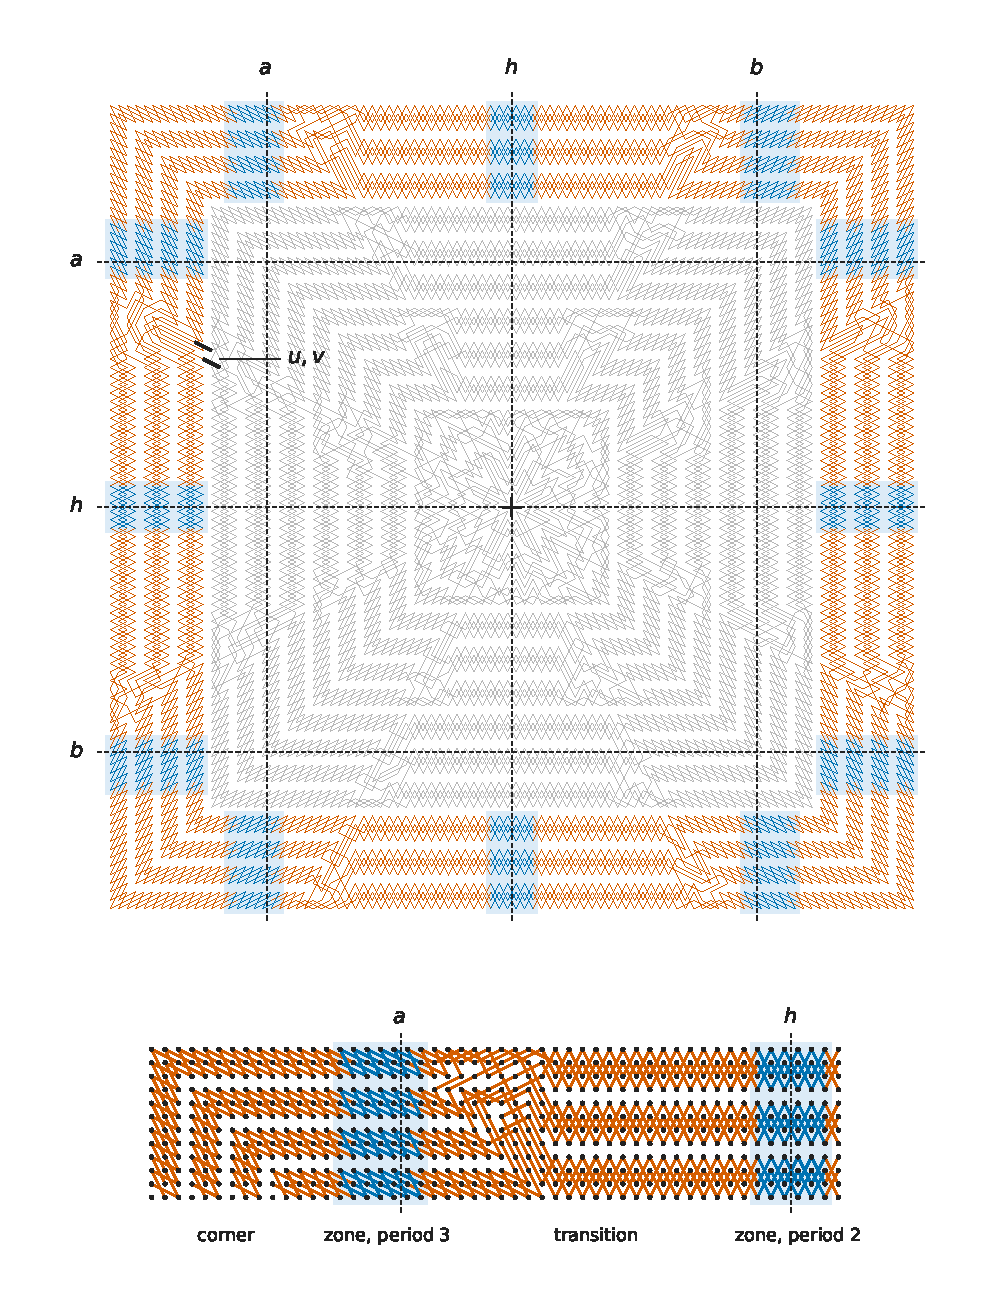
\includegraphics[width=0.78\textwidth]{ring96.pdf}
\caption{Top: the seed tour $T_1$ of side $96$. The inner board (grey) carries the tour $T_0$ of side $72$ except
for one arc; the short black arcs join its ends $u,v$ to the ring path. The shaded parts of the ring are the zones:
three intervals of columns on the top and bottom sides, and three intervals of rows on the left and right sides.
Dashed lines mark the cuts $a$, $h$, $b$ where rows and columns are inserted. Bottom:
the left half of the top side, enlarged.}
\label{fig:ring}
\end{figure}

\begin{remark}\label{rem:shape}
In all six seeds, and on all four sides, the moves in the zones follow one rule. Rotate the side to the top, so
that the path runs towards smaller columns, and let $i$ be the row. In the first zone the move is $(2,1)$ if
$i\equiv0\pmod3$ and $(-1,-2)$ otherwise. In the second it is $(2,-1)$ if $i\bmod4\in\{0,1\}$ and $(-2,-1)$
otherwise. In the third it is $(1,-2)$ if $i\bmod3\in\{0,1\}$ and $(-2,1)$ otherwise. So the path runs in lanes that
advance one column per move, in bands of three rows near the corners and of four rows in the middle. This explains
the shape of the construction, although the proof does not use it. A ring that fits both kinds of band has width
$12$, so the side grows by $24$ and six seeds are needed. The amounts $6e$, $12e$, $6e$ come from the geometry: in
centred coordinates the move $(2,1)$ is an arc only where $x>2y$, and the line $x=2y$ meets the top row $6$ columns
further from the corner each time the side grows by $24$.
\end{remark}

\section{Tours and computations}\label{sec:comp}

\subsection*{Search}
We followed Beluhov's formulation in \cite[answer 231]{knuth}, with a SAT solver in place of integer programming.
\begin{enumerate}
\item One Boolean variable per arc. Every cell has exactly one outgoing and one incoming arc.
\item For $24$ rays in generic directions, exactly $c$ chosen arcs cross each ray (a necessary condition by
Lemma~\ref{lem:rays}).
\item Solve. If the solution has more than one cycle, forbid each short cycle and its three rotations, and repeat.
\end{enumerate}
We used CaDiCaL~\cite{cadical} through PySAT~\cite{pysat}. Each tour below was found in at most a few minutes on a
laptop.

For $n/2$ coils and $n\ge72$ we searched for the ring only. The arcs of a known tour of side $n-24$ are kept on
the inner board, except that exactly one of them may be dropped, and the variables are the arcs at ring cells. For
the six seeds we added the requirements that in each zone, widened by one column on either side, the move depends
only on the depth of the cell, and that condition (S) holds. Each seed was then found in under a second. With
these zones the search reports that no seed exists for $N_1=82$, $88$ or $90$, at least over the inner tours that we
tried.

\subsection*{Calibration}
With the ray constraints removed or with $c$ fixed, exhaustive enumeration reproduces the counts of
\cite[answer 229]{knuth}: $2$ tours for $n=6$ (both with $5$ coils), $142$ for $n=7$ (all with $5$ coils), $1120$ for $n=8$
(all with $7$ coils) and $146$ for $n=9$ (all with $7$ coils). It finds no tour with $n$ coils for $4\le n\le8$, one for
$n=3$, and none with $n/2$ coils for $n=8$ and $n=10$.

\subsection*{Tours}
\begin{itemize}
\item \emph{$n$ coils.} $n=12,16,20,24,28,32,36,40,44,48$.
\item \emph{$n/2$ coils.} Every $n\equiv0$ or $2\pmod 8$ with $16\le n\le90$, that is, $20$ tours.
\item \emph{Seeds for $n/2$ coils.} $N_1=96,98,104,106,112,114$. Each contains the listed tour of side $N_1-24$
except for one arc.
\end{itemize}
The cell sequences accompany this note, in the files \texttt{tours\_n\_coils.txt},
\texttt{tours\_half\_coils.txt} and \texttt{seeds\_half\_coils.txt}. Figure~\ref{fig:tours} shows four of the
tours.

\begin{figure}[h]
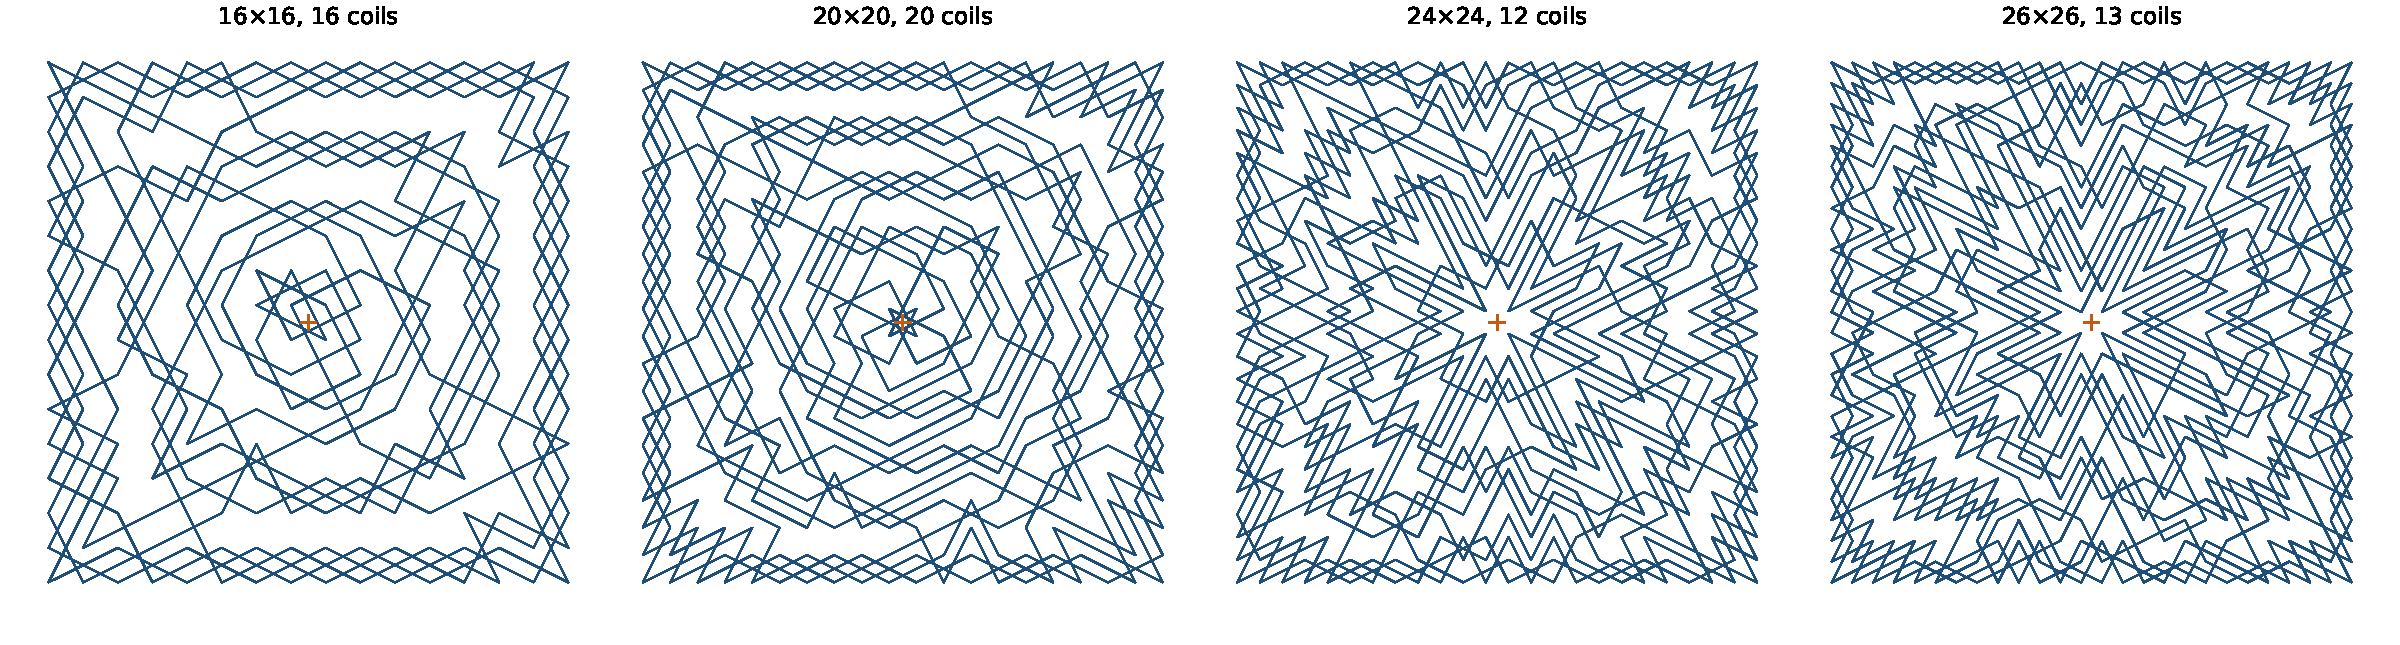
\includegraphics[width=\textwidth]{new_tours.pdf}
\caption{Whirling knight's tours. Left to right: $16\times16$ with $16$ coils, $20\times20$ with $20$ coils,
$24\times24$ with $12$ coils, $26\times26$ with $13$ coils. The cross marks the pivot.}
\label{fig:tours}
\end{figure}

\begin{table}[h]
\centering\small
\begin{tabular}{lrrrrrrrrrrrrrrrr}
\toprule
$n$ & 6 & 7 & 8 & 9 & 10 & 11 & 12 & 13 & 14 & 15 & 16 & 17 & 18 & 19 & 20 & 21\\
least $c$ & 5 & 5 & 7 & 7 & 7 & 7 & 8 & 8 & 9 & 9 & 8 & 10 & 9 & 10 & 12 & 12\\
\midrule
$n$ & 22 & 23 & 24 & 25 & 26 & 27 & 28 & 29 & 30 & 31 & 32 & 33 & 34 & 35 & 36 & 37\\
least $c$ & 13 & 13 & 12 & 13 & 13 & 15 & 16 & 16 & 17 & 17 & 16 & 18 & 17 & 19 & 20 & 20\\
\bottomrule
\end{tabular}
\caption{The least number of coils $c$ of an $n\times n$ whirling knight's tour, according to the SAT search. There
is no $5\times5$ tour.}
\label{tab:least}
\end{table}

\subsection*{The least number of coils for other $n$}
For $n\equiv0$ or $2\pmod 8$ the least number of coils is $n/2$, by Theorem~\ref{thm:half}. For the other $n$ we have
only computations. Table~\ref{tab:least} lists the least $c$ for which the search finds a tour, for $6\le n\le37$;
the tours are in the files \texttt{tours\_least\_coils.txt} and \texttt{tours\_half\_coils.txt}. For every smaller $c\ge n/2$ the solver reports that
there is no tour, and for $n\ge12$ it does so before any cycle has to be excluded. The entries for $n=6,7,8,9$ and
$11$ agree with the counts in \cite[answer 229]{knuth}. Beyond the table we found the following.
\begin{itemize}
\item \emph{$n\equiv4$ or $6\pmod 8$.} There are tours with $n/2+2$ coils for every such $n$ with $12\le n\le46$.
The solver reports none with $n/2+1$ coils for $12\le n\le36$.
\item \emph{Odd $n$.} There are tours with $(n+1)/2$ coils for $n=19$, $25$, $43$, $49$, $67$ and $73$. The solver
reports none for any other odd $n$ with $5\le n\le65$. For those $n$ with $13\le n\le47$ there are tours with $(n+3)/2$ coils.
\end{itemize}

\begin{question}\label{q:least}
Let $n\ge12$. Is the least number of coils of an $n\times n$ whirling knight's tour equal to $n/2+2$ when
$n\equiv4$ or $6\pmod 8$, to $(n+1)/2$ when $n\equiv1$ or $19\pmod{24}$, and to $(n+3)/2$ for every other odd $n$?
\end{question}
The appearance of the modulus $24$ for odd $n$ matches the ring construction of Section~\ref{sec:half}. A ring of
width $12$ can indeed be put around the tours of sides $25$ and $49$ with $13$ and $25$ coils, but our search found
none around the tours of sides $19$, $43$ and $67$ that we tried.

\subsection*{Verification}
\begin{itemize}
\item Every tour was checked by a separate program in exact rational arithmetic: each step is a knight move with
$u\times w>0$, every cell is visited once, and the number of plumb-line crossings is as stated.
\item The inequalities $g\le0$ and the values of the right-hand side in Lemma~\ref{lem:count} were also checked by
the accompanying program \texttt{verify\_weights.py}, in exact arithmetic, for every $n\le70$ not divisible by $4$.
\item Two further implementations, each written by a separate AI agent from the text of the proof alone, confirmed
the three cases up to $n=122$ and $n=130$.
\item For $13\le n\le27$, the Farkas certificates and three SAT solvers independently agree with
Theorem~\ref{thm:main}.
\item The program \texttt{half\_family.py} uses only the Python standard library. It checks conditions (Z), (S), (W)
and (C) for the six seeds. Independently of Proposition~\ref{prop:stretch}, it builds $T_k$ and checks it directly
as a tour. We ran this for $k\le20$ in each of the six families, which covers every admissible $n\le570$, and for
$n=1000$.
\item A third AI agent, which saw only this text and the data files, re-implemented the conditions and the
construction. It confirmed (Z), (S), (W), (C) for the six seeds and checked $T_k$ directly for every admissible $n$
from $72$ to $810$ and for $n=1000$. It also carried out the insertions of Lemma~\ref{lem:insert} one by one for
$e\le5$ and compared the result with the formula, and it tested the lemma on all $8458$ intervals of the six ring
paths that satisfy its hypotheses. By a separate exhaustive search it confirmed that no tour has $n/2$ coils for
$n=4,6,8,10,12,14$ and $20$. It found no mathematical error; its remarks on the exposition are incorporated.
\end{itemize}

\subsection*{Use of AI}
The search programs, the certificate search, the ring construction, the proofs and this manuscript were produced
with Claude (Anthropic) under the author's direction. The further implementations mentioned above were written by separate AI agents that
saw only the text of the proofs. The author is responsible for the content.

\begin{thebibliography}{9}
\bibitem{knuth} D.~E.~Knuth, \emph{The Art of Computer Programming}, Volume 4, Pre-Fascicle 8A: \emph{Hamiltonian
Paths and Cycles}, draft of 8 May 2026, exercises 7.2.2.4--227 to 232 and their answers.
\url{https://www-cs-faculty.stanford.edu/~knuth/fasc8a.ps.gz}
\bibitem{li} S.~Li, Nonexistence of whirling-knight tours at half coil count for $n\equiv4,6\pmod 8$,
arXiv:2605.04603 (2026).
\bibitem{cadical} A.~Biere, K.~Fazekas, M.~Fleury and M.~Heisinger, CaDiCaL, Kissat, Paracooba, Plingeling and
Treengeling entering the SAT Competition 2020, in \emph{Proc.\ SAT Competition 2020}, University of Helsinki, 2020.
\bibitem{pysat} A.~Ignatiev, A.~Morgado and J.~Marques-Silva, PySAT: a Python toolkit for prototyping with SAT
oracles, in \emph{SAT 2018}, LNCS 10929, Springer, 2018, 428--437.
\end{thebibliography}
\end{document}
